\section{Introduction}

\label{sec:intro}
Reconstructing a solid model from a scattered set of points is a common and well studied problem in computer graphics. 
Interest in this problem is rooted in the desire to convert real life data-sets -- data acquired from range scanners and now increasingly from commodity hardware like the Kinect -- to 3D polygonal models. 
It also has applications in model re-meshing and mesh hole filling, when one has a poorly structured mesh and would like a better representation of it. 

Given an oriented point-set, a common approach is to find an implicit function whose iso-contour corresponds to an approximation of the original surface. 
In this work we take a ``signal processing'' approach to this problem -- we cast the problem into a general shift-invariant setting. 
More explicitly, we reconstruct the desired implicit function within a space spanned by lattice translates of a single generating function. 
The extension to this class of function spaces allows us to anchor our basis functions at non-Cartesian lattice sites (\SC{sec:smpl_review}). Our approach is general and applicable to any valid lattice and generator, but our implementation is narrowed to applicable function spaces over the \emph{Body Centred Cubic} (BCC) and \emph{Cartesian} (CC) lattices.

\begin{figure*}
  \centering
  \mbox{} \hfill
	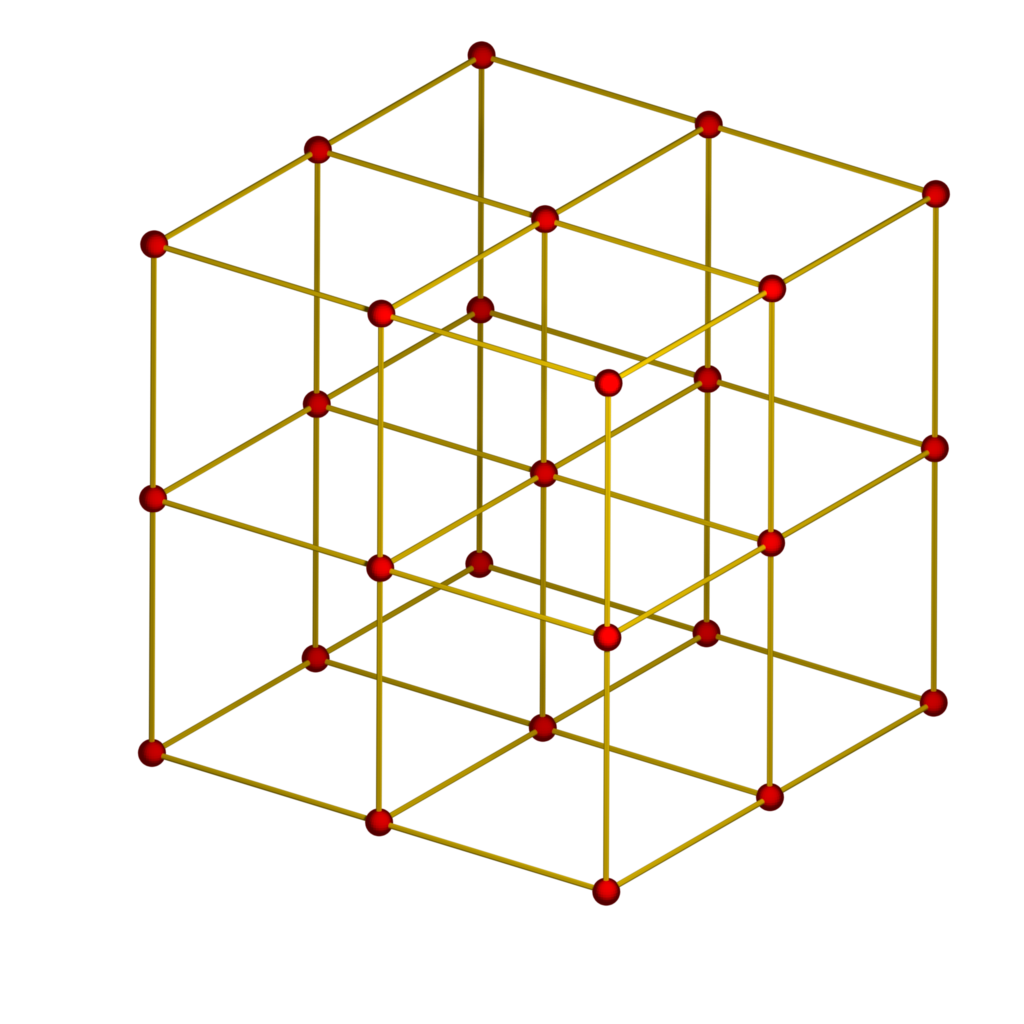
\includegraphics[width=.3\linewidth]{figures/lattice/cc}
	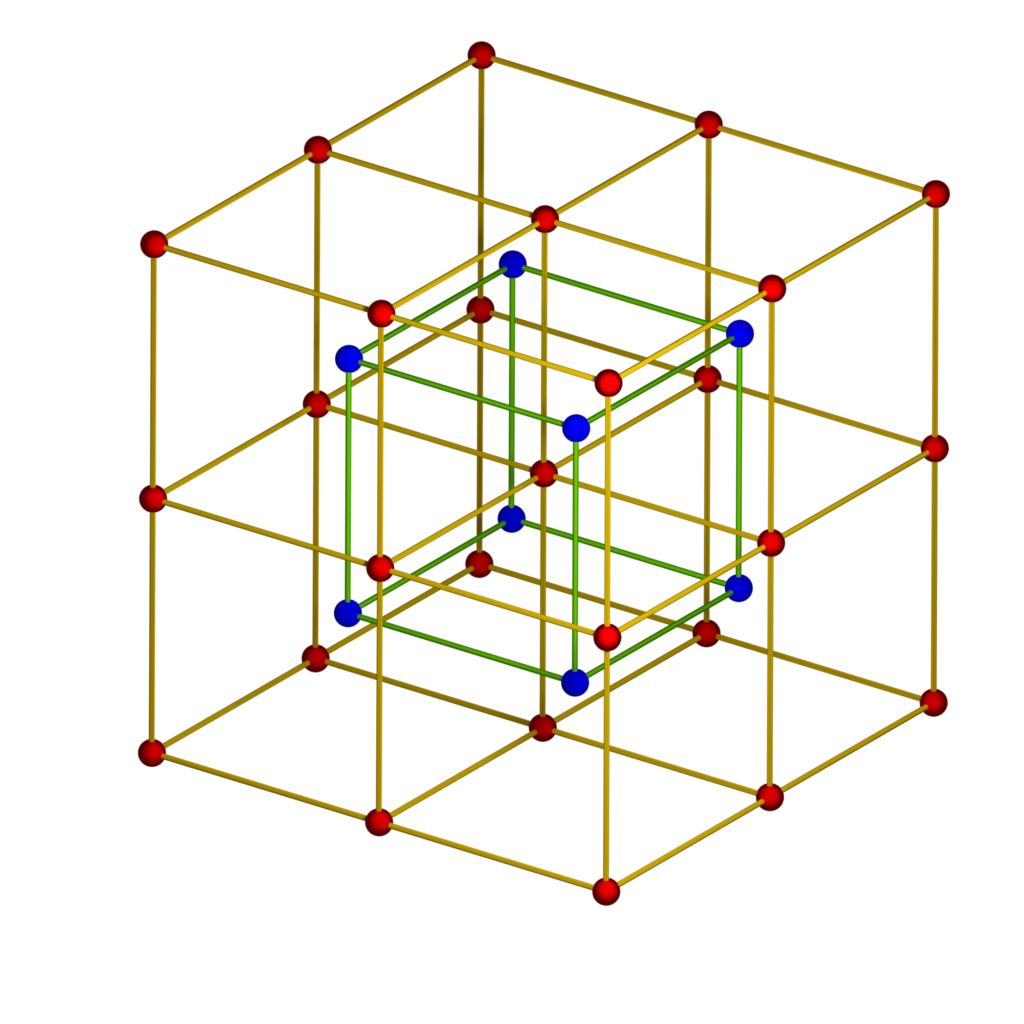
\includegraphics[width=.3\linewidth]{figures/lattice/bcc}
	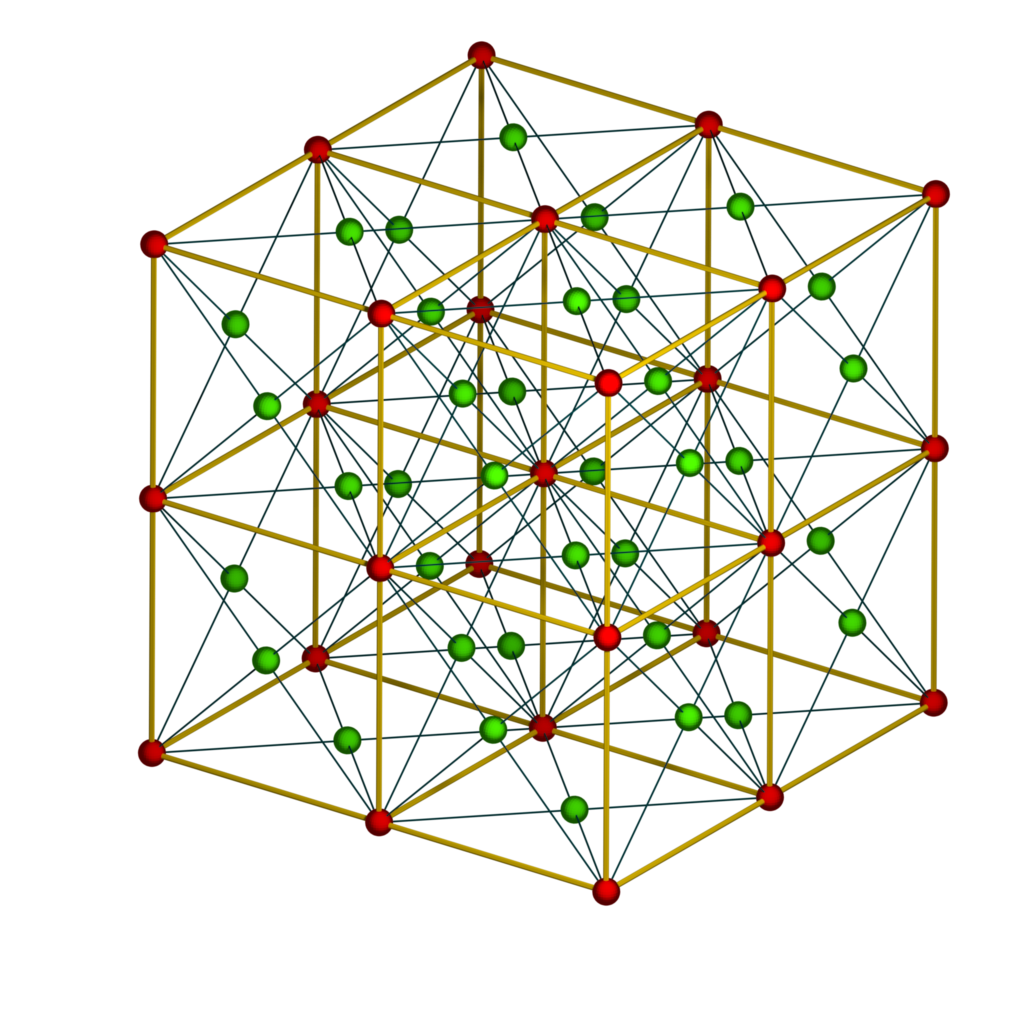
\includegraphics[width=.3\linewidth]{figures/lattice/fcc} \\
	
  \mbox{} \hfill
	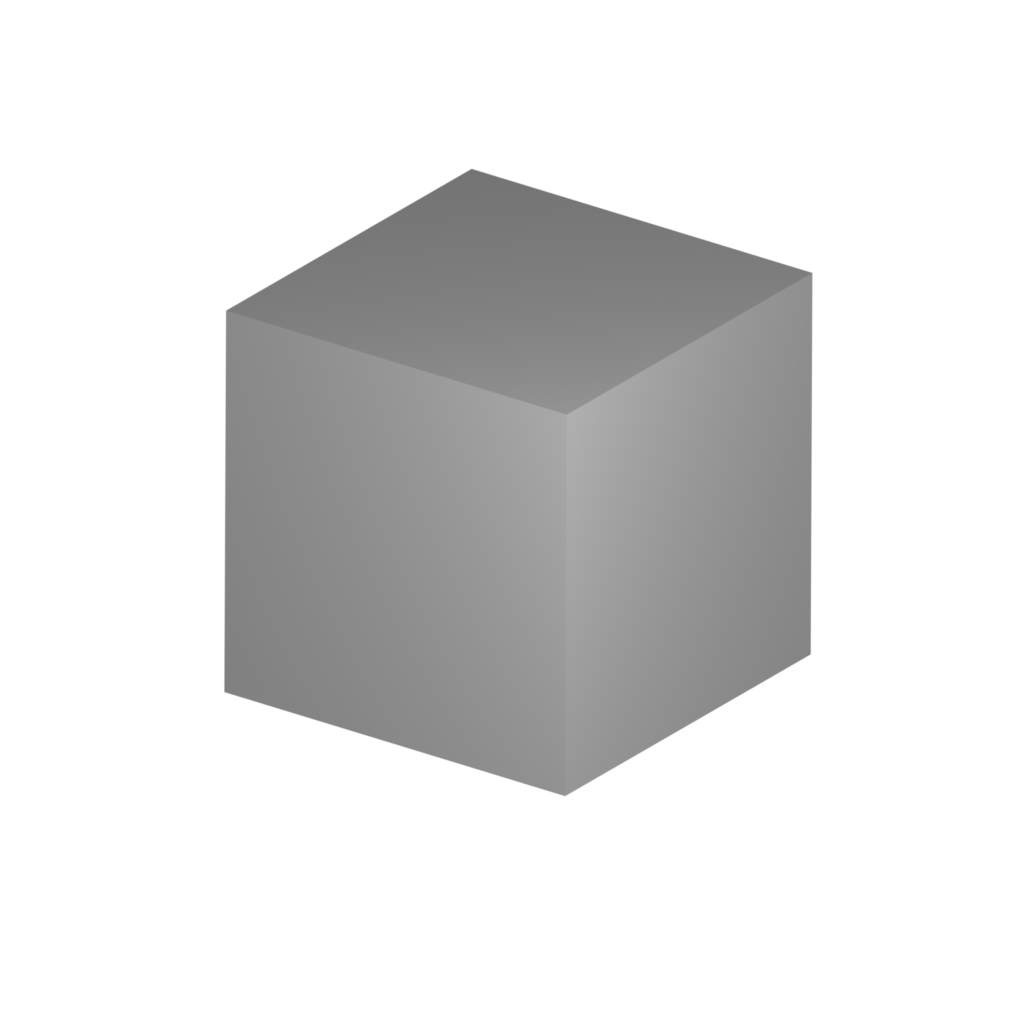
\includegraphics[width=.3\linewidth]{figures/lattice/cc_cell}
	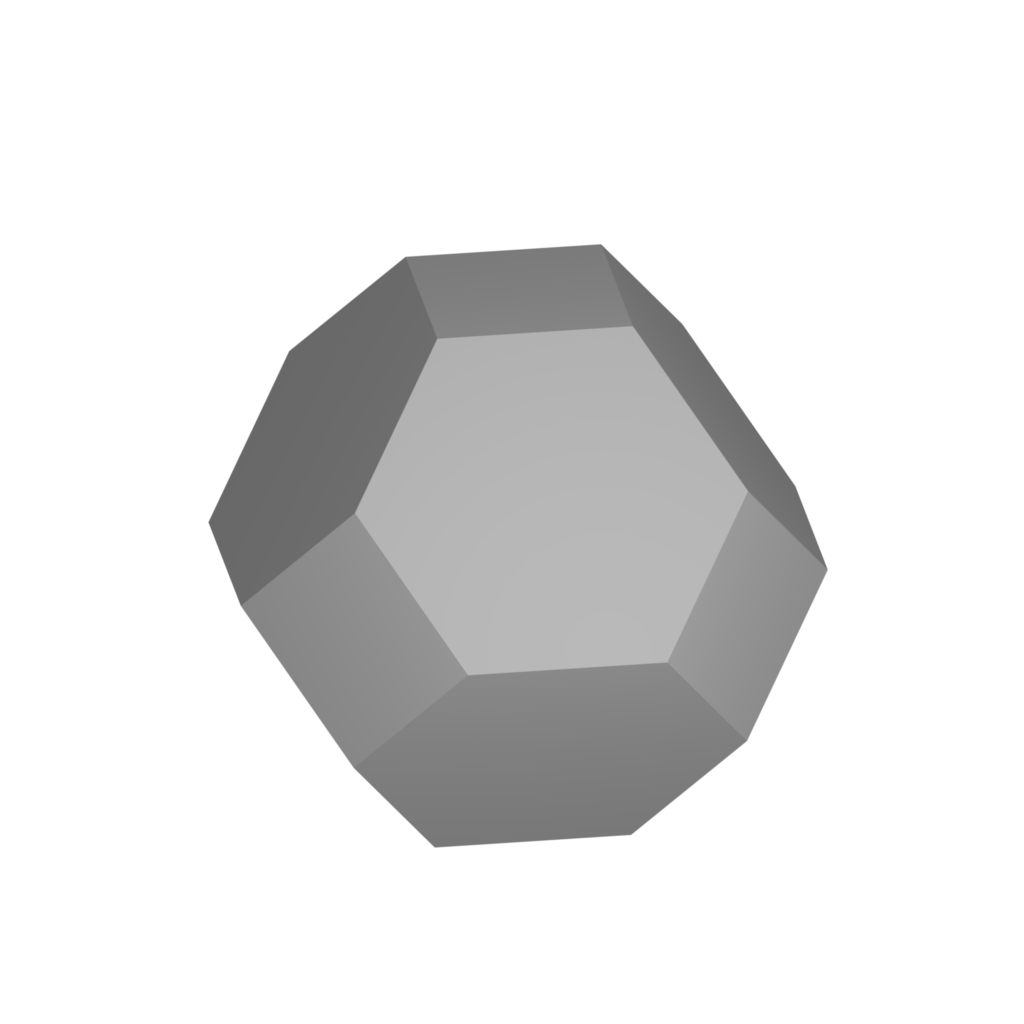
\includegraphics[width=.3\linewidth]{figures/lattice/bcc_cell}
	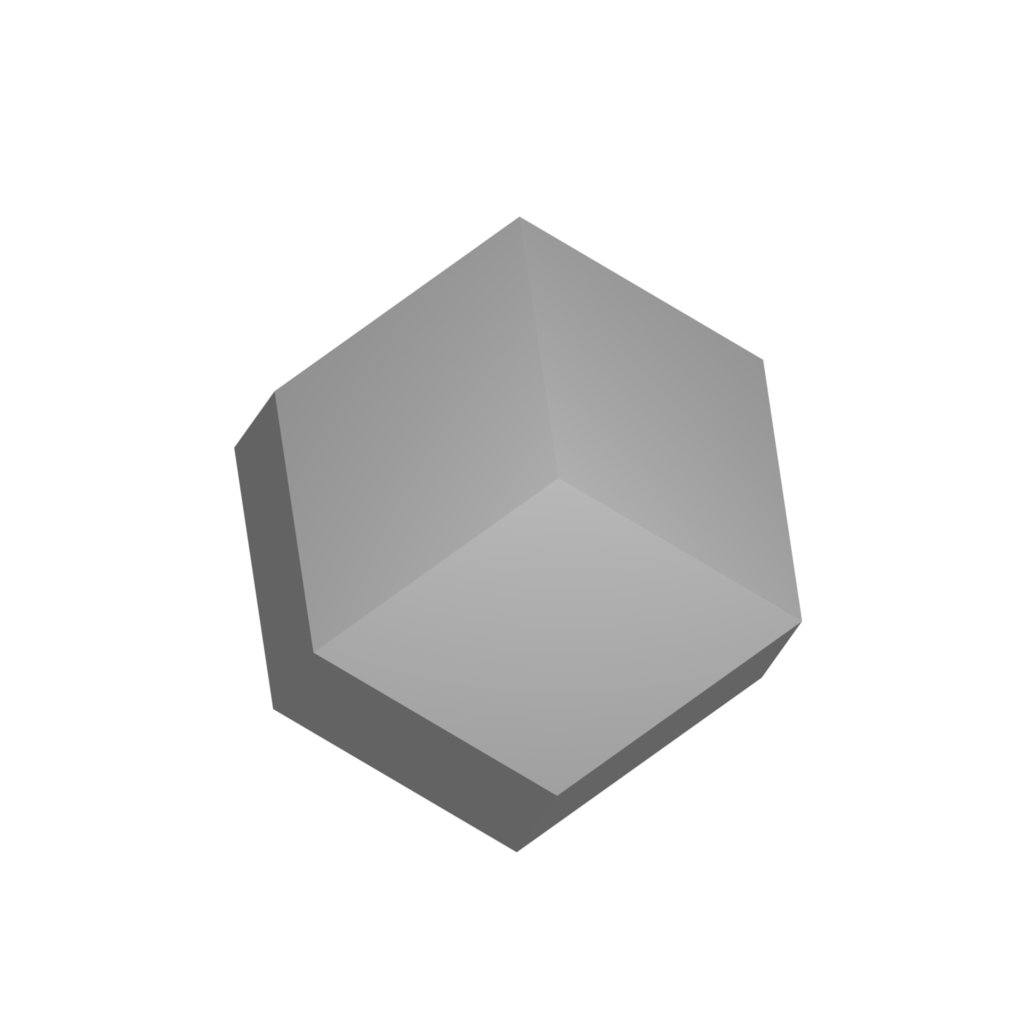
\includegraphics[width=.3\linewidth]{figures/lattice/fcc_cell} \\
   \hfill \mbox{}
  \caption{\label{fig:lattices}
  Sampling lattices (top) with with their corresponding Voronoi regions (bottom). Left to right are the CC, BCC and FCC lattices respectively.
  }
\end{figure*}

The advantage of moving to the BCC lattice is two fold. 
First, it's well known that the BCC lattice generates the optimal sampling pattern in $\realn^3$. 
The argument for optimality is simple; the sampling of a function with respect to the BCC lattice is equivalent to a periodization of it's Fourier frequency spectrum about the BCC's dual lattice, the \emph{Face Centered Cubic} (FCC) lattice.
Optimality follows from the observation that the FCC lattice is the optimal sphere packing lattice in three dimensions, that is, it packs frequency replica as tightly as possible in the Fourier domain, resulting in less \emph{pre-aliasing} from sampling. 
For isotropically band-limited functions, this tighter packing of frequency content allows for about 30\% more information to be captured when compared to samplings generated from a Cartesian lattice.
The second advantage to moving to the BCC lattice is that there exist reconstruction filters on the BCC lattice that outperform commonly used filters of equivalent order on the CC lattice in terms of both speed and accuracy \cite{practicalbox} (in software implementations) -- these filters are also more compact than their typical CC counterparts. 
In the context of our surface reconstruction scheme, this gives rise to regularization matrices that are more sparse on the BCC lattice and tend to provide faster convergence when optimizing the initial point set (\SC{sec:vari_review}).

Our surface reconstruction methodology follows the general Poisson approach, but with a few twists. 
First, we construct a smoothed approximation to the gradient field of a model's indicator function. 
We then estimate the divergence of that gradient field and feed it into a Poisson solver that outputs the coefficients needed to approximate the smoothed indicator function in a target shift invariant space. 
This Poisson solver is tailored to cater to the approximation power provided by each space. 
However, our approach is novel in two notable ways. 
Firstly, we employ a variational scheme to obtain a lattice-based approximation of the gradient field. 
This scheme depends only on the generating kernel of the target space and optimizes a functional that incorporates interpolation and smoothness constraints. 
Secondly, we utilize the theory behind shift-invariant spaces to seek discretizations of the divergence and Laplacian operators that are tailored to exploit the full approximation capabilities of the target space.

Additionally, we consider the possibility of approximating the smoothed gradient field representation within function spaces that are spanned by shifted versions of a single generating kernel. 
In the context of gradient estimation, introducing a shift in the direction of the derivative has shown to improve overall gradient approximation fidelity in terms of gradient orientation and magnitude, as well as displaying the ability to capture higher frequency details that are smoothed out in non-shifted schemes~\cite{gradrev}. 
Since the divergence operator is intimately connected to the gradient operator, these results are of interest to us. Using an appropriate discretization of the derivative/divergence operator is an important step in recovering the indicator function of the initial model. We also derive specific error bounds, based on an error kernel formulation, for approximations of linear operators in arbitrary shift invariant spaces.

To summarize, our contributions are as follows:
\begin{itemize}
\item[$\bullet$] We reformulate the Poisson surface reconstruction approach using general shift-invariant spaces as the target approximation space
\item[$\bullet$] Specifically, we investigate the reconstruction of surfaces in both a sub-optimal (Cartesian) and an optimal (BCC)
  box-spline function space
\item[$\bullet$] We present a new variational resampling scheme that resamples the original scattered oriented points' normals onto any regular lattice. This resampling scheme depends on the generating kernel, but is general enough to be extended to shifted generating kernels as this has been shown to improve gradient estimation in shift invariant spaces. 
\item[$\bullet$] We present an extension of the error kernel of Blu and Unser to general linear operators and show how to design filters that respect the full approximation order of the target approximation space.
\item[$\bullet$] While our focus is on comparing the surface reconstruction algorithm on both the CC and BCC lattices, we also provide qualitative and quantitative comparisons between the presented technique (on both the Cartesian and BCC lattices) and similar methods. 
\end{itemize}


